% !TEX program = xelatex
\documentclass[UTF8,zihao=-4,oneside,openany]{ctexbook}

% Shared style for the combined handout.  Section files keep standalone
% preambles for now, while the master document uses this single definition.
\usepackage[a4paper,top=20mm,bottom=22mm,left=19mm,right=19mm,headheight=24pt]{geometry}
\usepackage[table]{xcolor}
\usepackage{amsmath,amssymb,mathtools,bm}
\usepackage{siunitx}
\usepackage{booktabs,tabularx,array,multicol}
\usepackage{enumitem}
\usepackage{tikz}
\usetikzlibrary{arrows.meta,positioning,calc,angles,quotes,patterns}
\usepackage[most]{tcolorbox}
\usepackage{fancyhdr}
\usepackage{hyperref}

\definecolor{Ink}{HTML}{202326}
\definecolor{DeepBlue}{HTML}{294E69}
\definecolor{Blue}{HTML}{47687D}
\definecolor{PaleBlue}{HTML}{F3F5F6}
\definecolor{Gold}{HTML}{6E777D}
\definecolor{PaleGold}{HTML}{F6F6F5}
\definecolor{Green}{HTML}{5B6D76}
\definecolor{PaleGreen}{HTML}{F3F5F6}
\definecolor{Alert}{HTML}{666B6F}
\definecolor{PaleAlert}{HTML}{F6F6F6}
\definecolor{RuleGray}{HTML}{D3D7DA}
\definecolor{TextGray}{HTML}{61686D}
\definecolor{SoftGray}{HTML}{F6F6F6}

\color{Ink}
\sisetup{
  per-mode=symbol,
  inter-unit-product=\ensuremath{{}\cdot{}},
  exponent-product=\times
}

\hypersetup{
  colorlinks=true,
  linkcolor=DeepBlue,
  urlcolor=Blue,
  pdfsubject={高中物理竞赛一轮资料重排讲义},
  pdfauthor={物理竞赛一轮资料编写组}
}

\setlength{\parindent}{2em}
\setlength{\parskip}{0.25em}
\setlist{nosep,leftmargin=2em}
\setcounter{secnumdepth}{3}
\setcounter{tocdepth}{2}
\numberwithin{equation}{section}
\counterwithin{table}{section}
\allowdisplaybreaks[2]
\emergencystretch=2em

\ctexset{
  chapter={
    format=\raggedright\LARGE\bfseries\color{Ink},
    titleformat=\LARGE\bfseries\color{Ink},
    beforeskip=0pt,
    afterskip=18pt
  },
  section={
    format=\Large\bfseries\color{DeepBlue},
    beforeskip=1.8ex,
    afterskip=1.0ex
  },
  subsection={
    format=\large\bfseries\color{Ink},
    beforeskip=1.5ex,
    afterskip=0.8ex
  },
  subsubsection={format=\normalsize\bfseries\color{Ink}}
}

\pagestyle{fancy}
\fancyhf{}
\fancyhead[L]{\small\color{TextGray}高中物理竞赛一轮讲义}
\fancyhead[R]{\small\color{TextGray}第一章\quad 数学与物理工具}
\fancyfoot[C]{\small\color{TextGray}\thepage}
\renewcommand{\headrulewidth}{0.4pt}
\renewcommand{\headrule}{\hbox to\headwidth{\color{RuleGray}\leaders\hrule height \headrulewidth\hfill}}

\newcommand{\dimens}[1]{\operatorname{dim}\!\left(#1\right)}
\newcommand{\dd}{\mathop{}\!\mathrm{d}}
\newcommand{\vect}[1]{\bm{#1}}
\newcommand{\uvec}[1]{\hat{\vect{#1}}}
\newcommand{\e}{\mathrm e}
\newcommand{\order}[1]{\mathcal O\!\left(#1\right)}
\DeclareMathOperator{\proj}{proj}
\newcommand{\examplesource}[1]{%
  \par{\small\color{TextGray}题源：#1}\par
}

\newtcolorbox{goalbox}{
  enhanced,breakable,
  colback=PaleBlue,colframe=Blue,
  boxrule=0.7pt,arc=2mm,
  title={本节目标},fonttitle=\bfseries,
  coltitle=DeepBlue,
  attach boxed title to top left={xshift=5mm,yshift=-2mm},
  boxed title style={colback=white,colframe=Blue,boxrule=0.7pt,arc=1.5mm}
}

\newtcolorbox{sourcebox}{
  enhanced,breakable,
  colback=SoftGray,colframe=RuleGray,
  boxrule=0.5pt,arc=0mm,
  title={题源说明},fonttitle=\bfseries,
  coltitle=Ink,colbacktitle=SoftGray,
  borderline west={1.2pt}{0pt}{TextGray}
}

\newtcolorbox[auto counter,number within=section]{examplebox}[2][]{
  enhanced,breakable,
  colback=white,colframe=RuleGray,
  boxrule=0.5pt,arc=0mm,
  title={例题~\thetcbcounter\quad #2},fonttitle=\bfseries,
  coltitle=Ink,colbacktitle=PaleBlue,
  borderline west={1.4pt}{0pt}{DeepBlue},
  #1
}

\newtcolorbox{methodbox}[1]{
  enhanced,breakable,
  colback=PaleBlue,colframe=RuleGray,
  boxrule=0.5pt,arc=0mm,
  title={方法：#1},fonttitle=\bfseries,
  coltitle=Ink,colbacktitle=PaleBlue,
  borderline west={1.2pt}{0pt}{DeepBlue}
}

\newtcolorbox{warningbox}[1]{
  enhanced,breakable,
  colback=SoftGray,colframe=RuleGray,
  boxrule=0.5pt,arc=0mm,
  title={易错提醒：#1},fonttitle=\bfseries,
  coltitle=Ink,colbacktitle=SoftGray,
  borderline west={1.2pt}{0pt}{TextGray}
}

\newtcolorbox{extensionbox}[1]{
  enhanced,breakable,
  colback=PaleGold,colframe=Gold,
  boxrule=0.5pt,arc=0mm,
  title={拓展：#1},fonttitle=\bfseries,
  coltitle=Ink,colbacktitle=PaleGold,
  borderline west={1.2pt}{0pt}{DeepBlue}
}

\newtcolorbox{summarybox}{
  enhanced,breakable,
  colback=PaleBlue,colframe=DeepBlue,
  boxrule=0.9pt,arc=1.5mm,
  title={本节小结},fonttitle=\bfseries,
  coltitle=white,colbacktitle=DeepBlue
}

\newtcolorbox{exercisebox}[1]{
  enhanced,breakable,
  colback=white,colframe=RuleGray,
  boxrule=0.7pt,arc=1.5mm,
  title={#1},fonttitle=\bfseries,
  coltitle=DeepBlue,colbacktitle=PaleBlue
}

\tikzset{
  vector/.style={-{Latex[length=2.5mm]},very thick,draw=DeepBlue},
  component/.style={-{Latex[length=2.2mm]},thick,draw=TextGray},
  axis/.style={-{Latex[length=2mm]},thin,draw=TextGray},
  guide/.style={densely dashed,draw=TextGray},
  curve/.style={very thick,draw=DeepBlue},
  tangent/.style={thick,draw=TextGray},
  secant/.style={thick,draw=DeepBlue}
}


\hypersetup{
  pdftitle={高中物理竞赛一轮讲义：第一章第一节 力的基本性质（含解答与解图）},
  pdfsubject={以学而思一轮资料为基础重新组织，并补写完整解答}
}

\fancyhead[R]{\small\color{TextGray}第一章\quad 静力学}
\renewcommand{\theequation}{\thechapter.\arabic{equation}}

\newtcolorbox{origexamplebox}[1]{
  enhanced,
  colback=white,colframe=RuleGray,
  boxrule=0.5pt,arc=0mm,
  title={#1},fonttitle=\bfseries,
  coltitle=Ink,colbacktitle=PaleBlue,
  borderline west={1.4pt}{0pt}{DeepBlue}
}

\newenvironment{xesolution}{%
  \par\smallskip
  \begingroup\small
  \noindent{\bfseries\color{DeepBlue}解答}\quad
}{%
  \par\endgroup\medskip
}

\begin{document}

\pagenumbering{arabic}
\setcounter{page}{1}
\chapter{静力学}

同学们可能有所耳闻，自然界中有四种基本的相互作用力，它们分别是万有引力、电磁力、
强和弱相互作用力。力（force）是物体之间相互作用的一种表现形式，当有力作用在任何一个
物体上时，它将会对力的作用产生响应，响应的形式有很多，其中最明显的就是运动状态或
形状的改变。我们将首先学习力的基本的一面，即如何对力进行测量，如何描写物质系统的
受力，在已知力作用下处于静止状态力学系统的性质。在随后的课程中将逐步深入，研究在
已知的力作用下如何预测物体未来的运动的方法，从力的宏观性质出发进入到物质世界的深处
进一步探索力的起源。

\section{力的基本性质}

对宏观物体受力的研究是学习描写各种力最初的一步，将来可以看到，这里所学的技术对于
那些无法直观体验的对象之间相互作用的问题提供了丰富的术语和方法。为了完整描写宏观
物体所受的一个力，需要指出该力的大小、方向和作用在物体上的位置，也就是作用点，它们
合起来称为力的三要素。从更基本的观点来看，力可以用空间中的一个矢量来描写，力的三要素
一起给出了作为一个矢量的大小、方向和起点的位置。方向和作用点由传统的几何方法给出，
而力的大小则需要引入一个新的单位，为了纪念力学的奠基人，今天将力的单位取为牛顿，
用 N 来表示，将在动力学中给出其准确含义。

虽然从最基本的角度来看自然界只有四种相互作用力，而且强、弱相互作用只存在于亚原子
物理当中，也就是说宏观物体的受力全部起源于万有引力和电磁相互作用力，原则上可以根据
它们的性质以及物质的结构从微观理论出发预测出各种情况下宏观物体的受力。但是实践上以
这种方法得到宏观物体的受力实际上是不现实的，因为物质世界极大的复杂性。所以在实际的
研究过程中首先根据力的表现形式和效果对其进行分类，研究力和那些已知的、容易观察的物理量
之间的关系，最后逐步地深入探讨力的本质和起源。基于经验和观察人们发现了几种常见的力，
下面我们逐一了解一下它们。

\clearpage
\subsection{重力}

本质上讲重力是万有引力在地球表面附近的一种表现形式，它来自于地球对所有物体的吸引。
观测表明，处于地球表面附近的物体都会受到重力作用，在地球的任何地方，其方向均竖直
向下指向地面，大小正比于物体的质量，作用于物体的重心处。关于重力有几点需要说明的地方：

\begin{itemize}
  \item 将地表任何一点处物体所受重力大小 $G$ 与其质量 $m$ 的比例系数称为地表的重力
  加速度，用 $g$ 表示
  \begin{equation}
    G=mg,\qquad g\approx\SI{9.8}{\metre\per\second\squared}.
  \end{equation}

  \item 真实测量表明，地表各处的 $g$ 并不完全相同。纬度、海拔、地球形状和自转
  都会带来修正；在大多数近地竞赛题中，这些差异可以忽略。

  \item 近地问题中把重力方向定义为当地铅垂向下。它一般不严格指向地心，但在小尺度问题中
  可视为方向和大小都不变的均匀场。

  \item 在均匀重力场中，各部分所受重力的合力作用线通过质心，因而重心与质心重合。
  如果物体可以看成
  是由多个质点构成，将这些质点编号，第 $i$ 个质点的质量为 $m_i$，在固定的直角坐标系中
  的位置为 $(x_i,y_i,z_i)$ 时，质心的坐标 $(x_c,y_c,z_c)$ 为
  \begin{equation}
    x_c=\frac{\sum_i m_ix_i}{\sum_i m_i},\qquad
    y_c=\frac{\sum_i m_iy_i}{\sum_i m_i},\qquad
    z_c=\frac{\sum_i m_iz_i}{\sum_i m_i}.
  \end{equation}
\end{itemize}

\begin{origexamplebox}{例 1.1}
求一块三边长分别为 $a,b,c$ 的均匀三角板的重心位置。

\begin{center}
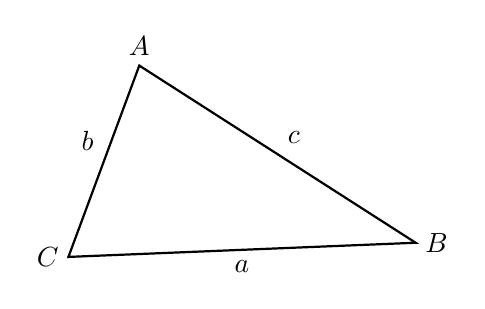
\begin{tikzpicture}[scale=0.9]
  \coordinate (A) at (0.6,2.7);
  \coordinate (B) at (4.5,0.2);
  \coordinate (C) at (-0.4,0);
  \draw[thick] (A)--node[above right] {$c$}(B)--node[below] {$a$}(C)--node[above left] {$b$}cycle;
  \node[above] at (A) {$A$};
  \node[right] at (B) {$B$};
  \node[left] at (C) {$C$};
\end{tikzpicture}
\end{center}
\end{origexamplebox}

\begin{xesolution}
取三角形三个顶点的位置矢量分别为 $\vec r_A,\vec r_B,\vec r_C$。先作一条中线，例如从
$A$ 连到 $BC$ 的中点 $D$。把三角板分成平行于 $BC$ 的许多极细长条，每个长条的质心都在
$AD$ 上，因而整块板的质心也在 $AD$ 上。同理，它还在其他中线上，所以质心就是三条中线的交点 $G$。

\begin{center}
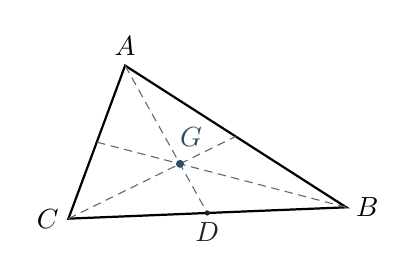
\begin{tikzpicture}[scale=0.72]
  \coordinate (A) at (0.6,2.7); \coordinate (B) at (4.5,0.2); \coordinate (C) at (-0.4,0);
  \coordinate (D) at ($(B)!0.5!(C)$); \coordinate (E) at ($(C)!0.5!(A)$);
  \coordinate (F) at ($(A)!0.5!(B)$); \coordinate (G) at (barycentric cs:A=1,B=1,C=1);
  \draw[thick] (A)--(B)--(C)--cycle;
  \draw[guide] (A)--(D) (B)--(E) (C)--(F);
  \fill[Ink] (D) circle (1.3pt) node[below] {$D$};
  \fill[DeepBlue] (G) circle (2pt)
    node[above=6pt,xshift=4pt,inner sep=0pt] {$G$};
  \node[above] at (A) {$A$}; \node[right] at (B) {$B$}; \node[left] at (C) {$C$};
\end{tikzpicture}
\end{center}

中线交点将每条中线按从顶点起 $2:1$ 分割，等价地
\[
  \boxed{\vec r_G=\frac{\vec r_A+\vec r_B+\vec r_C}{3}}.
\]
边长 $a,b,c$ 只决定三角形的形状，不改变“重心为中线交点”这一结论。
\end{xesolution}

\begin{origexamplebox}{例 1.2}
求由三根均匀杆构成的三角形的重心位置，其中三杆长度分别为 $a,b,c$，满足
$a^2+b^2=c^2$。分别用 $\lambda_a,\lambda_b,\lambda_c$ 表示各杆的线密度，先求一般结果，
再讨论三杆线密度相同的情形。

\begin{center}
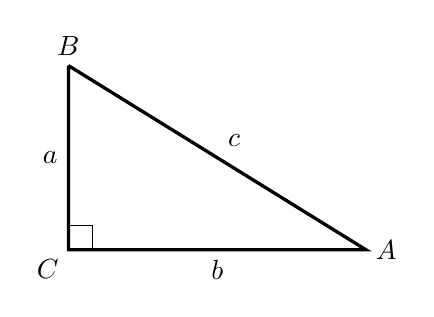
\begin{tikzpicture}[scale=0.9]
  \coordinate (C) at (0,0);
  \coordinate (B) at (0,2.6);
  \coordinate (A) at (4.2,0);
  \draw[very thick] (B)--node[left] {$a$}(C)--node[below] {$b$}(A)--node[above right] {$c$}(B);
  \draw[thin] (0,0.34)--(0.34,0.34)--(0.34,0);
  \node[above] at (B) {$B$};
  \node[below left] at (C) {$C$};
  \node[right] at (A) {$A$};
\end{tikzpicture}
\end{center}
\end{origexamplebox}

\begin{xesolution}
“均匀”表示每根杆内部的线密度不随位置变化，并不表示三根杆的线密度一定相等。
取直角顶点 $C$ 为原点，$CA$ 沿 $x$ 轴、$CB$ 沿 $y$ 轴。
三根杆的质量及各自中点为
\[
\begin{array}{c|c|c}
\text{杆} & \text{质量} & \text{质心坐标}\\ \hline
BC & \lambda_a a &(0,a/2)\\
CA & \lambda_b b &(b/2,0)\\
AB & \lambda_c c &(b/2,a/2)
\end{array}
\]
记总质量为 $M=\lambda_a a+\lambda_b b+\lambda_c c$。各杆的质量乘其质心坐标后相加，得到
\[
 Mx_G=\lambda_a a\cdot0+\lambda_b b\cdot\frac b2+\lambda_c c\cdot\frac b2,
\]
\[
 My_G=\lambda_a a\cdot\frac a2+\lambda_b b\cdot0+\lambda_c c\cdot\frac a2.
\]
所以一般结果为
\[
 \boxed{x_G=\frac{b(\lambda_b b+\lambda_c c)}{2M},\qquad
 y_G=\frac{a(\lambda_a a+\lambda_c c)}{2M}}.
\]
只有进一步给定 $\lambda_a=\lambda_b=\lambda_c=\lambda$，才可约去共同线密度，得到
\[
  \boxed{x_G=\frac{b(b+c)}{2(a+b+c)},\qquad
  y_G=\frac{a(a+c)}{2(a+b+c)}} ,
\]
其中 $c=\sqrt{a^2+b^2}$。这里不能套用“三角板的中线交点”：面密度均匀与线密度均匀是两个不同的质量分布。
式中分子量纲为质量乘长度、分母为质量，坐标的量纲正确。若某一杆的质量远大于另外两杆，
一般式便趋于该杆中点的坐标，也符合质心的含义。
\end{xesolution}

\begin{origexamplebox}{例 1.3}
求下面阴影的重心。

\begin{center}
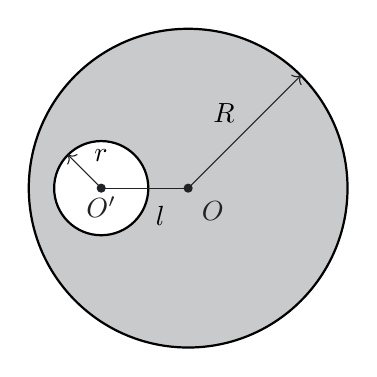
\begin{tikzpicture}[scale=0.92]
  \coordinate (O) at (0.70,0);
  % Leave a visible annular gap: the sketch has R=2.20, r=0.65, l=1.20.
  \coordinate (Op) at (-0.50,0);
  \fill[TextGray!35,even odd rule] (O) circle (2.20) (Op) circle (0.65);
  \draw[thick] (O) circle (2.20);
  \draw[thick] (Op) circle (0.65);
  \fill[Ink] (O) circle (1.8pt) node[below right=2pt] {$O$};
  \fill[Ink] (Op) circle (1.8pt)
    node[below=3pt,inner sep=0pt] {$O'$};
  \draw[->,draw=Ink] (O)--++(45:2.20) node[midway,above left] {$R$};
  \draw[->,draw=Ink] (Op)--++(135:.65) node[midway,above right] {$r$};
  \draw[draw=Ink] (Op)--(O) node[pos=0.68,below=3pt] {$l$};
\end{tikzpicture}
\end{center}
\end{origexamplebox}

\begin{xesolution}
设薄片面密度为 $\sigma$，以大圆圆心 $O$ 为原点。把挖去的小圆看成位于 $O'$ 的“负质量”，则
\[
  M=\sigma\pi R^2,\qquad m=\sigma\pi r^2.
\]
剩余部分的质量为 $M-m$，对 $O$ 取质量矩，
\[
  (M-m)\vec r_G=M\vec 0-m\,\overrightarrow{OO'}.
\]
所以
\[
  \boxed{\vec r_G=-\frac{r^2}{R^2-r^2}\,\overrightarrow{OO'}}.
\]
\begin{center}
\begin{tikzpicture}[scale=0.62]
  \coordinate (O) at (0,0);
  \coordinate (Op) at (-0.92,0);
  \coordinate (G) at (0.42,0);
  \fill[TextGray!30,even odd rule] (O) circle (1.75) (Op) circle (0.52);
  \draw[thick] (O) circle (1.75);
  \draw[thick] (Op) circle (0.52);
  \draw[guide] (Op)--(G);
  \fill[Ink] (Op) circle (1.6pt);
  \draw[thin,TextGray] (Op)--(-1.92,0);
  \node[left=2pt,inner sep=0pt] at (-1.92,0) {$O'$};
  \fill[Ink] (O) circle (1.6pt) node[below=3pt] {$O$};
  \fill[DeepBlue] (G) circle (2pt) node[above right=2pt] {$G$};
  \draw[-{Latex[length=2.2mm]},thick,draw=DeepBlue]
    ($(O)+(0,0.34)$)--($(G)+(0,0.34)$)
    node[midway,above] {$\vec r_G$};
  \node[font=\scriptsize,text=TextGray,anchor=west] at (1.95,0.35)
    {质心在小孔的反方向};
  \draw[guide] (1.85,0.20)--(0.55,0.06);
\end{tikzpicture}\\[-0.4ex]
{\scriptsize\color{TextGray}方向示意；为便于辨认，图中 $OG$ 的长度未按比例绘制。}
\end{center}
质心位于 $OO'$ 直线上、在小孔的反方向，与 $O$ 的距离为
$lr^2/(R^2-r^2)$。这一结果要求小圆孔完全位于大圆内，即 $l+r\le R$。
\end{xesolution}

\begin{origexamplebox}{例 1.4}
已知一个质量为 $M$ 的没有盖子的圆柱形的杯子。里面开始是空的，然后往里面慢慢地注水。
进入了杯子的水和杯子的总重心会发生变化。请问重心如何变化？是否有最值？是多少？
（已知杯子底面积为 $S$，水的密度为 $\rho$，原来空杯子重心高度为 $H$，杯内允许的
最大水深为 $h_{\max}$。）
\end{origexamplebox}

\begin{xesolution}
设水面高度为 $h$，从杯底向上量取坐标。水的质量为 $\rho Sh$，其质心高度为 $h/2$，
因而系统质心高度为
 \begin{equation}
  z(h)=\frac{MH+\frac12\rho Sh^2}{M+\rho Sh}.
  \label{eq:cup-centre-mass}
\end{equation}
\begin{center}
\begin{tikzpicture}[scale=0.68]
  \fill[PaleBlue] (0.06,0.06) rectangle (2.64,1.45);
  \draw[very thick] (0,3.10)--(0,0)--(2.70,0)--(2.70,3.10);
  \draw[thick,draw=DeepBlue] (0.06,1.45)--(2.64,1.45);
  \draw[guide] (1.35,0)--(1.35,3.10);
  \draw[<->,draw=Ink] (-0.36,0)--(-0.36,1.45)
    node[midway,left] {$h$};
  \fill[Ink] (1.35,0.725) circle (1.7pt);
  \draw[guide] (1.45,0.725)--(3.08,0.725);
  \node[anchor=west,inner sep=0pt] at (3.12,0.725)
    {水的质心：$h/2$};
  \draw[Ink,thick] (1.27,2.48)--(1.43,2.64) (1.27,2.64)--(1.43,2.48);
  \draw[guide] (1.45,2.56)--(3.08,2.56);
  \node[anchor=west,inner sep=0pt] at (3.12,2.56)
    {空杯重心：$H$};
  \fill[DeepBlue] (1.35,1.86) circle (2pt);
  \draw[guide] (1.45,1.86)--(3.08,1.86);
  \node[anchor=west,inner sep=0pt,text=DeepBlue] at (3.12,1.86)
    {总质心：$z(h)$};
\end{tikzpicture}\\[-0.4ex]
{\scriptsize\color{TextGray}某一注水状态示意；$z(h)$ 总在 $H$ 与 $h/2$ 之间，图中具体高度不代表一般大小关系。}
\end{center}
注水时新加入的一层水位于高度 $h$，由式 \eqref{eq:cup-centre-mass} 也可直接得到
\[
  \frac{\dd z}{\dd h}=\frac{\rho S}{M+\rho Sh}\,[h-z(h)].
\]
因此，当新加水层低于当前质心时，质心下降；高于当前质心时，质心上升。极小值满足 $z(h_*)=h_*$，即
\[
  \frac12\rho S h_*^2+Mh_*-MH=0.
\]
取正根得
\[
  \boxed{h_*=z_{\min}
  =\frac{\sqrt{M^2+2M\rho SH}-M}{\rho S}}.
\]
结合题设给出的最大水深，可达的最低重心为
\[
  \boxed{z_{\min,\text{可达}}=
  \begin{cases}
    h_*, & h_{\max}\ge h_*,\\[2pt]
    \displaystyle\frac{MH+\frac12\rho S h_{\max}^2}
    {M+\rho S h_{\max}}, & h_{\max}<h_*.
  \end{cases}}
\]
第二种情形中，$0\le h\le h_{\max}$ 内有 $h<z(h)$，所以 $z(h)$ 始终随注水下降，
最小值确在装到 $h_{\max}$ 时取得。
\end{xesolution}

\begin{origexamplebox}{例 1.5【思考题】}
已知一个均匀质量的圆球壳，半径为 $R$，现在将球壳上端高度为 $h$ 的部分切下，然后
粘贴在圆球的最下面，形成一个“杯子”。求这个杯子的重心。
\end{origexamplebox}

\begin{xesolution}
以原球心为原点，向上为 $z$ 轴。这里的“粘贴在圆球的最下面”是指：
球冠保持原来的朝向，不作翻转，整体向下平移，使球冠顶点与原球壳最低点粘接；
球冠的圆形边缘位于最下方，构成杯子的底座。

\begin{center}
\begin{tikzpicture}[scale=0.82]
  \begin{scope}[shift={(-3.30,0)}]
    % 取示意半径 1.5、球冠高度 0.5；切口在 y=1.0。
    \draw[thick]
      (-1.12,1.00) arc[start angle=138.2,end angle=401.8,radius=1.50];
    \draw[very thick,DeepBlue]
      (-1.12,1.00) arc[start angle=138.2,end angle=41.8,radius=1.50];
    \draw[guide] (-1.12,1.00)--(1.12,1.00);
    \draw[guide] (-1.62,0)--(1.62,0);
    \draw[guide] (0,-1.65)--(0,1.75) node[above=1pt]{$z$};
    \draw[<->] (-1.72,1.50)--(-1.72,1.00) node[midway,left]{$h$};
    \fill[Ink] (0,0) circle (1.5pt) node[below right]{$O$};
    \node[DeepBlue,font=\small] at (0,-1.90) {(1) 切下上球冠};
  \end{scope}
  \draw[-{Latex[length=2.3mm]},thick,draw=TextGray] (-1.25,0.05)--(1.25,0.05);
  \node[font=\scriptsize,align=center,inner sep=0pt] at (0,0.72)
    {不翻转\\整体下移 $2R$};
  \begin{scope}[shift={(3.30,0.45)}]
    % 原球壳上方开口；灰虚线仅标出球冠原来的位置。
    \draw[thick]
      (-1.12,1.00) arc[start angle=138.2,end angle=401.8,radius=1.50];
    \draw[TextGray,dashed]
      (-1.12,1.00) arc[start angle=138.2,end angle=41.8,radius=1.50];
    \draw[guide] (-1.12,1.00)--(1.12,1.00);
    \draw[guide] (-1.62,0)--(1.62,0);
    \draw[guide] (0,-2.30)--(0,1.70) node[above=1pt]{$z$};
    % 同一球冠向下平移 2R：顶点恰好接触原球壳最低点。
    \draw[very thick,DeepBlue]
      (-1.12,-2.00) arc[start angle=138.2,end angle=41.8,radius=1.50];
    % 圆形切口的透视示意：前半实线、后半虚线。
    \draw[DeepBlue,thick]
      (-1.12,-2.00) arc[start angle=180,end angle=360,x radius=1.12,y radius=0.12];
    \draw[DeepBlue,thick,densely dashed]
      (-1.12,-2.00) arc[start angle=180,end angle=0,x radius=1.12,y radius=0.12];
    \fill[Ink] (0,0) circle (1.5pt) node[below right]{$O$};
    \fill[DeepBlue] (0,-1.50) circle (1.7pt);
    \draw[TextGray,thin] (0,-1.50)--(1.68,-1.12)--(1.92,-1.12);
    \node[font=\scriptsize,anchor=west,inner sep=0pt]
      at (1.96,-1.12) {粘接点};
    \draw[DeepBlue,thin] (1.12,-2.00)--(1.48,-2.25);
    \node[DeepBlue,font=\scriptsize,anchor=west,inner sep=0pt]
      at (1.50,-2.25) {圆形支承边缘};
    \node[DeepBlue,font=\small] at (0,-2.82) {(2) 作为底座粘贴};
  \end{scope}
\end{tikzpicture}
\\[-0.4ex]
{\scriptsize\color{TextGray}蓝色曲线表示同一球冠；右图中球冠在原球壳外部，顶点与球壳最低点相接。}
\end{center}

设球壳面密度为 $\sigma$。高为 $h$ 的薄球冠面积为 $2\pi Rh$，而对球壳水平分层有
$\dd A=2\pi R\,\dd z$，所以球冠质心高度为
\[
  z_c=\frac{\int_{R-h}^{R}z\,\dd z}{\int_{R-h}^{R}\dd z}
  =R-\frac h2.
\]
球冠原来的顶点坐标为 $R$。平移后该顶点与原球壳最低点 $-R$ 重合，
所以整个球冠向下平移了 $2R$，其质心的新坐标为
\[
  z_c'=z_c-2R=-R-\frac h2.
\]
球冠质量 $m_c=2\pi Rh\sigma$，原球壳总质量 $M_0=4\pi R^2\sigma$。
取下原位置的球冠，再把它粘到新位置，系统质量不变；相对于原球壳，质量矩的改变量为
\[
  M_0z_G=-m_cz_c+m_cz_c'
  =m_c(z_c'-z_c)=-2Rm_c.
\]
因此
\[
  z_G=\frac{-2R(2\pi Rh\sigma)}{4\pi R^2\sigma}
  =\boxed{-h}.
\]
负号表示杯子的重心在原球心下方，距原球心为 $h$。这个结果也可直接理解为：
占总质量 $h/(2R)$ 的球冠整体下降了 $2R$，所以系统质心下降 $h$。
\end{xesolution}

\subsection{弹力}

当相互接触的物体发生形变时所产生的恢复形变的力称为弹性力，胡克定律表明，当物体
形变不太大时，弹性力与形变成正比，弹簧的弹性力 $F$ 与弹簧相对于原长的形变（拉伸
或压缩）$x$ 成正比。取沿弹簧轴的有符号形变量 $x$，弹力分量与形变反向，即
\begin{equation}
  F=-kx,
\end{equation}
式中比例系数 $k$ 称为弹簧的倔强系数，也叫劲度系数，负号表示弹性力与形变反方向。
这里形变为零的位置对应弹簧原长，不一定是物体受所有外力后的平衡位置。例如竖直弹簧
悬挂物体时，平衡伸长量为 $mg/k$，该处弹力仍向上且大小为 $mg$，并不为零。
关于弹力也有几点需要注意的地方：

\begin{itemize}
  \item 当把多根弹簧并排放置共同作用时，称两弹簧并联，并联弹簧在任意位置处形变量
  相同。这里取共同连接到刚性横杆上的理想轻弹簧，讨论沿弹簧轴的小形变：共同位移为 $x$，
  第 $i$ 根弹簧提供的力为 $F_i=k_i x$，故总力为
  \[
    F=\sum_iF_i=\left(\sum_i k_i\right)x.
  \]
  与 $F=kx$ 比较，多根弹簧并联的等效劲度系数为
  \begin{equation}
    k=k_1+k_2+\cdots,
  \end{equation}
  为每根弹簧劲度系数之和。和电路类比，除了并联以外多根弹簧之间也可以串联，处于串联
  状态的弹簧在受力以后形变量并不相同；连接点质量可忽略且无其他外力时，各弹簧的张力相同。
  把各段伸长量相加，可得串联弹簧的等效劲度
  系数为
  \begin{equation}
    \frac1k=\frac1{k_1}+\frac1{k_2}+\cdots.
  \end{equation}

  \item 绳子的张力是一种弹性力，绳子和与之连接的物体之间有相互作用时，不仅绳子与
  物体之间有弹性力，而且在绳子内部也因发生相对形变而出现弹性力。这时，绳子上任一
  横截面两边互施作用力，这对作用力和反作用力称为绳子的张力，一般情况下，与绳子相应
  的比例系数 $k$ 很大，因而形变很小，可以忽略。所以绳子的张力不是由绳子的形变规律
  确定，而是由求解力学问题时确定。因而我们一般抽象出柔软不可伸长的轻绳。

  \item 物体与支撑面接触时，微观形变会产生接触力。接触力的法向分量称为支持力 $N$；
  只在光滑面模型中，合接触力才必定沿曲面法线。若表面粗糙，还要加上沿切平面的摩擦力，
  此时合接触力通常不与表面垂直。支持力和摩擦力的大小不是预先给定的，而由运动状态与约束共同决定。

  \item 所有弹力的起源均为电磁相互作用力，这一点只有从微观角度才能够发现。
\end{itemize}

\begin{origexamplebox}{例 1.6}
证明：串联弹簧的等效弹性系数小于其中任何一根弹簧的弹性系数，并解释形成这一现象的原因。
\end{origexamplebox}

\begin{xesolution}
两根弹簧串联时张力相同，设为 $F$。各弹簧伸长量为 $x_i=F/k_i$，总伸长量为
\[
  x=\sum_i x_i=F\sum_i\frac1{k_i}.
\]
令 $F=k_{\rm eq}x$，得
\[
  \frac1{k_{\rm eq}}=\sum_i\frac1{k_i}.
\]
因为对任意一根弹簧 $j$ 都有
\[
  \frac1{k_{\rm eq}}=\frac1{k_j}+\sum_{i\ne j}\frac1{k_i}>\frac1{k_j},
\]
所以
\[
  \boxed{k_{\rm eq}<k_j\qquad(\text{对所有 }j)}.
\]
物理上，同一个力使每根弹簧都伸长，而串联组的总伸长是各伸长量之和；与任意一根单独弹簧相比，
同力下形变更大，等效劲度自然更小。
\end{xesolution}

\subsection{滑动摩擦力、静摩擦力}

摩擦力也是一种接触力，当相互接触的物体作相对运动或有相对运动趋势时，接触面间会
产生一种阻碍相对运动或相对运动趋势的力，这种力称为摩擦力，前者称为滑动摩擦力，
后者称为静摩擦力。测量结果表明：

\begin{enumerate}[label=\arabic*.]
  \item 在库仑摩擦的近似模型中，滑动摩擦力大小与法向支持力成正比，方向与接触面上的相对滑动速度相反：
  \begin{equation}
    \vec f_k=-\mu_kN\frac{\vec v_{\rm rel}}{|\vec v_{\rm rel}|},
  \end{equation}
  其中 $\mu_k$ 称为动摩擦因数。“与表观接触面积无关”和“$\mu_k$ 为常数”都是一定条件下的理想化，
  不是对所有材料和速度都精确成立的定律。

  \item 在高中竞赛的常规库仑模型中，滑动摩擦力大小取为 $\mu_kN$，不再显式依赖速度大小。

  \item 静摩擦力是一个由平衡或共同运动条件决定的约束力，其大小满足
  \begin{equation}
    0\le |f_s|\le \mu_sN.
  \end{equation}
  只有在临界滑动时才取等号。$\mu_s$ 是最大静摩擦因数，与 $\mu_k$ 应当区分；若题目只给一个
  $\mu$，需根据所讨论的阶段明确它表示哪一个摩擦因数。
\end{enumerate}

\begin{origexamplebox}{例 1.7}
如图所示，木板 $A$ 质量为 $M$，以相对地面的速度 $v$ 在水平面上向北运动，木板上放
一质量为 $m$ 的板 $B$，各接触面间滑动摩擦因数均为 $\mu$，当木块 $B$ 也有相对地面
向东的速度 $v$ 时，试分析木块 $B$ 的受摩擦力的情况。

\begin{center}
\begin{tikzpicture}[x=1.0cm,y=1.0cm]
  \draw[fill=PaleBlue,draw=Ink,thick] (-2.5,-1.55) rectangle (2.5,1.55);
  \draw[fill=white,draw=Ink,thick] (-0.65,-0.4) rectangle (0.65,0.4);
  \node at (0,0) {$B$};
  \node[anchor=north west] at (-2.30,1.34) {$A$};
  \draw[vector] (2.9,-0.45)--(2.9,1.15) node[above] {$v$};
  \draw[vector] (-0.15,-0.72)--(1.45,-0.72) node[right] {$v$};
  \node[right] at (3.35,0.7) {北};
  \node[below] at (1.25,-1.02) {东};
\end{tikzpicture}
\end{center}
\end{origexamplebox}

\begin{xesolution}
取向东为 $x$ 正方向、向北为 $y$ 正方向。板 $A$ 和块 $B$ 对地速度分别为
\[
  \vec v_A=v\,\hat{\boldsymbol j},\qquad
  \vec v_B=v\,\hat{\boldsymbol i}.
\]
因而 $B$ 相对 $A$ 的滑动速度为
\[
  \vec v_{B/A}=\vec v_B-\vec v_A
  =v(\hat{\boldsymbol i}-\hat{\boldsymbol j}),
\]
方向为东南。$A$ 对 $B$ 的滑动摩擦力必须阻碍这个相对滑动，所以指向西北。

\noindent\begin{minipage}[c]{0.42\linewidth}
\centering
\begin{tikzpicture}[scale=0.64]
  \draw[axis] (-2.2,0)--(2.3,0) node[right]{东};
  \draw[axis] (0,-1.8)--(0,2.1) node[above]{北};
  \draw[vector] (0,0)--(1.4,0) node[below right]{$\vec v_B$};
  \draw[vector] (0,0)--(0,1.4) node[above left]{$\vec v_A$};
  \draw[component] (0,0)--(1.4,-1.4) node[below right]{$\vec v_{B/A}$};
  \draw[vector] (0,0)--(-1.15,1.15) node[above left]{$\vec f_{A\to B}$};
\end{tikzpicture}
\end{minipage}\hfill
\begin{minipage}[c]{0.55\linewidth}
若 $B$ 在竖直方向无加速度，则 $N=mg$，故
\[
  \boxed{\vec f_{A\to B}
  =\frac{\mu_kmg}{\sqrt2}
  (-\hat{\boldsymbol i}+\hat{\boldsymbol j})},
  \qquad |\vec f_{A\to B}|=\mu_kmg.
\]
摩擦力的方向要根据\textbf{相对速度}判断，不能只看 $B$ 的对地速度。
\end{minipage}
\end{xesolution}

\end{document}
